\section{Flow matching with path integral is able to discover latent Hellinger RDM}

\subsection{Embedding low-dimensional latent to high dimensional space}

Many experiments require observations $x \in \mathbb{R}^{d}$ while a simple generative model lives in a low-dimensional latent space $\mathbb{R}^{m}$ with $m \ll d$. To generate such kind of dataset, we use \emph{participation-ratio} (PR) regularized autoencoder to project low-dimensional dataset into high-dimensional dataset.

The PR-regularized autoencoder learns a deterministic map that lifts $z \in \mathbb{R}^{m}$ to embeddings $h \in \mathbb{R}^{d}$ without collapsing $h$ onto a very thin subspace of $\mathbb{R}^{d}$.
Fix $d \ge m$ and parameters $\psi$ for an encoder $f_{\psi}:\mathbb{R}^{m}\to\mathbb{R}^{d}$ and decoder $g_{\psi}:\mathbb{R}^{d}\to\mathbb{R}^{m}$; write
\begin{equation}
  h = f_{\psi}(z) \in \mathbb{R}^{d},
  \qquad
  \hat{z} = g_{\psi}(h) \in \mathbb{R}^{m}.
\end{equation}
Reconstruction is measured by mean squared error between $\hat{z}$ and $z$ over training samples.

Given a mini-batch of embeddings $h^{(1)},\ldots,h^{(n)}$, center them coordinatewise, let $\tilde{H}\in\mathbb{R}^{n\times d}$ have rows $(h^{(i)} - \bar{h})^{\mathsf{T}}$, and form the unbiased batch covariance $C = \frac{1}{n-1}\tilde{H}^{\mathsf{T}}\tilde{H}$.
The \emph{participation ratio} is
\begin{equation}
  \label{eq:pr-def}
  \mathrm{PR}(C) = \frac{\bigl(\operatorname{tr} C\bigr)^{2}}{\operatorname{tr}(C^{2}) + \varepsilon},
\end{equation}
with $\varepsilon>0$ a small numerical floor; larger $\mathrm{PR}(C)$ indicates that batch variance spreads across more directions in $\mathbb{R}^{d}$.
The training loss combines reconstruction and encouraging high participation,
\begin{equation}
  \label{eq:pr-loss}
  \mathcal{L}
  =
  \frac{1}{n}\sum_{i=1}^{n} \bigl\lVert g_{\psi}(f_{\psi}(z^{(i)})) - z^{(i)} \bigr\rVert_{2}^{2}
  - \lambda\,\mathrm{PR}(C),
\end{equation}
with $\lambda \ge 0$ trading fidelity to $z$ against spreading mass in the embedding space.

\subsection{Flow matching with path integral is able to discover latent Hellinger RDM}

We constructed two datasets. The latent datasets were constructed same as the previous notes, using gaussian tuning with random amplitude, and acitivty-modulated noise. We constructed 2D and 10D datasets, and embedded into higher dimensional space using PR-regularized autoencoder. We then used flow matching to estimate the Hellinger RDM, and found it is able to discover the latent Hellinger RDM.

\FloatBarrier
\begin{figure}[!htbp]
  \centering
  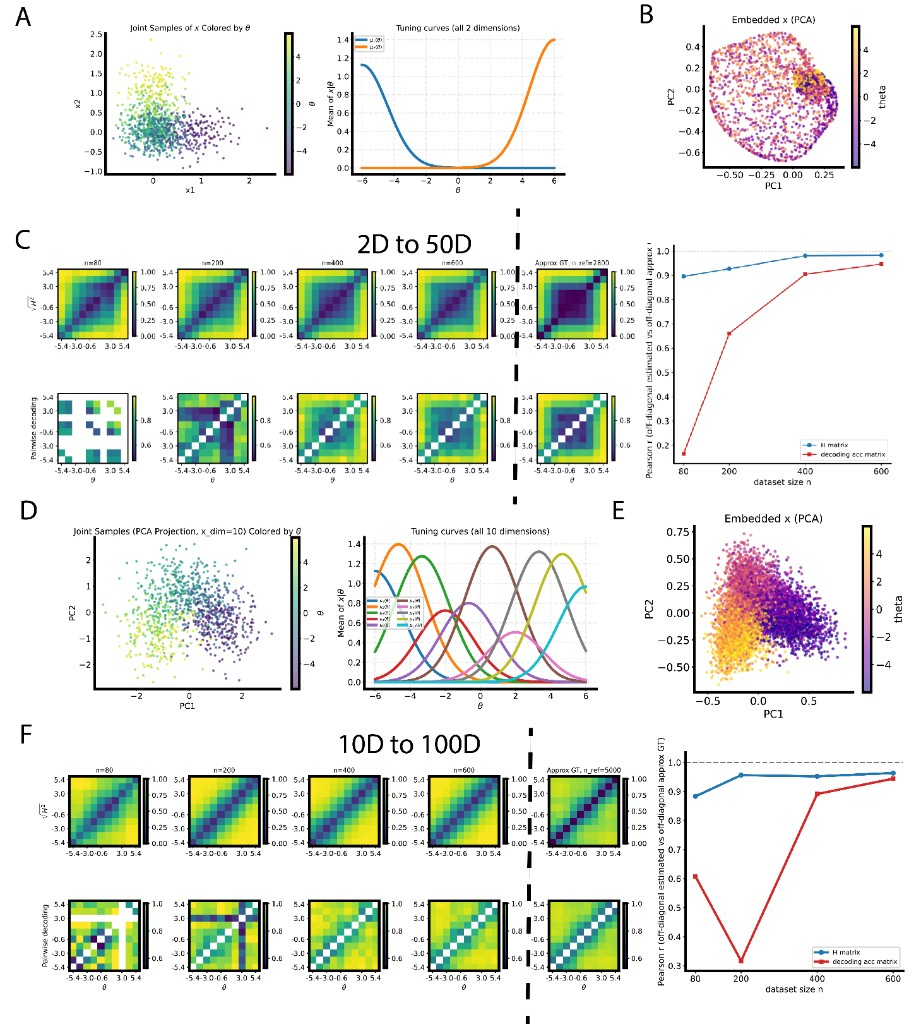
\includegraphics[width=\linewidth]{notes/figures/2026-04-20-pr-regularized-autoencoder/pr_embedding_theta_flow_h_decoding.png}
  \caption{%
  (A) 2D latent dataset. (B) Embedding to 50D using PR-regularized autoencoder, then visualized using PCA. (C) Flow matching is able to discover the latent Hellinger RDM. The GT was estimated based on the latent dataset only. (D, E, F) Same as A, B, C, but from 10D latent to 100D embedded space.
    }
  \label{fig:pr-embed-theta-path-integral-h-decoding}
\end{figure}